\section{Research Methods}

%   How can I assess the quality of my Methods section? To make a self-assessment of your Methods section, you can ask yourself the following questions.
%    * Have I really described my Methods in a way that is easy for readers to follow and which would enable them to replicate my work? Have I ensured that I have covered every step? Is my structure clear and complete?
%    * Have I been as concise as possible? Have I used references to previous works rather than repeating descriptions that readers could easily find elsewhere?
%    * Do the individual sentences in each paragraph contain too many, too few, or just the right manageable number of steps? Have I ensured that my sentences don’t sound like lists?
%    * Have I thought about the way readers prefer to receive information? (no ambiguity, no back referencing, everything in chronological order, headings, bullets)?
%    * Have I checked my grammar (infinitive, gerund, allow, thus etc.) with regard to how I outline how and why I made certain choices?
%    * Have I checked my journal’s guidelines on how to use numbers?
%    * Have I used tenses correctly? past simple (in the passive form to describe what I did), present simple (descriptions of established scientific fact)

This study performed a systematic literature review (SLR), contemplating the usage of Machine Learning techniques for code smells identification. SLRs are reviews organized and based on a clear search strategy, that ensures the rigor, completeness and reproducibility of the process, focusing on the identification, evaluation and interpretation of the available research that is relevant to a particular question~\citep{kitchenham2010systematic}.

In order to accomplish the SLR the following steps were taken: planning, defining research questions, searching databases, discussion of validity, data extraction, and synthesis of the results, those steps are in accordance to the typical steps taken for a SLR~\citep{keele2007guidelines}. The following subsections embrace each of those steps.

\subsection{Planning}

We developed a SLR protocol in order to assure that the research is executed in a planned way and not driven by the researcher expectations. In the protocol the following items were addressed as part of the planning for the study: research objectives; research questions; search strategy; study selection criteria and procedures; data extraction; and data classification strategies.

\subsection{Research Questions}

 The given review focuses on the "Identification of the best machine learning techniques for code smell detection", in order to accomplish that the following questions must be addressed

\begin{itemize}
    \item \textbf{RQ 1:} Which code smells are addressed when using Machine Learning techniques for the identification?
    RQ1 focuses on the identification of code smells that are more aimed by the literature. It can help identify which smells have not been employed and can be used as gaps for future works.
    \item \textbf{RQ 2:} Which Machine Learning techniques are used when identifying code smells?
    RQ2 aims in the identification of which Machine Learning are commonly used for this end, helping to identify potential techniques that were not yet explored for this end.
    \item \textbf{RQ 3:} Which Machine Learning techniques are most used for each kind of code smell?
    RQ3 is concerned with the relationship between the Machine Learning techniques and the code smells, allowing the identification of which techniques are more used for each code smells, it can also lead us to identify potential techniques that can be used for other smells that have not been covered yet.
    \item \textbf{RQ 4:} Which Machine Learning techniques performs better for each smell?
    RQ4 compares the performance of different techniques for the same code smell, providing evidence to identify models that have outstanding performance.
\end{itemize}

\subsection{Research Strategy}

In order to find relevant relationships between machine learning techniques and code smells in the literature, searches were conducted in four electronic databases - Science Direct, IEEE Xplorer, Wiley and ACM - for papers published until 2016. The definition of the search terms was done following these steps:
\begin{enumerate}
    \item{Derive major terms from research questions.}
    \item{Break down the major term in smaller terms.}
    \item{Identify alternative spellings or synonyms for the identified terms.}
    \item{Check the search terms in relevant papers we have.}
    \item{Use the Boolean OR to combine alternative spellings and synonyms. Use the Boolean AND to link major terms.}
\end{enumerate}

The following search applied for each database, taking the attention to adapt them for each library rules: "("code smell" OR "bad smell") AND ("learning" OR "data mining" OR "artificial intelligence" OR "pattern recognition" OR "case based reasoning" OR "decision tree" OR "regression tree" OR "classification tree" OR "neural net" OR "genetic programming" OR "genetic algorithm" OR "Bayesian belief network" OR "Bayesian net" OR "association rule" OR "support vector machine" OR "support vector regression")". This filter returned 1021 papers, distributed as shown in Figure \ref{fig:librariesImage}. The search string tries to filter papers that applies Machine Learning techniques for code smell identification problems.

\begin{figure}[hbt] 
	\caption{Distribution of papers by article}
	\label{fig:librariesImage}
	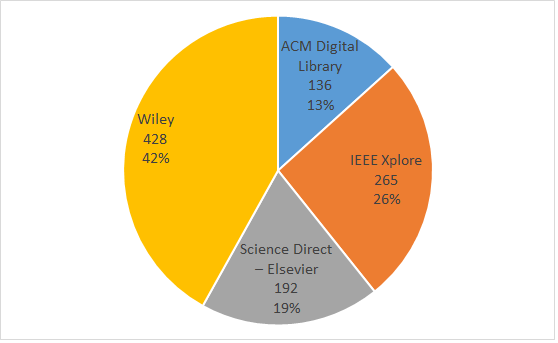
\includegraphics[width=0.95\textwidth]{imagens/librariesDistributionImage.png}
\end{figure}

After the filtering, 338 duplicated results were removed, resulting in 683 remaining results. Following to that publications which were not papers or proceedings papers which belonged to a Journal that is not related to Computational Fields were removed and, leaving 286 results left. The studies were then filtered by the publication title, removing any study which was not related to the usage of Machine Learning techniques for code smells identification, what left 155 results. This same criteria was applied when filtering by abstract, resulting in 53 papers left for classification. These steps were summarized in Figure \ref{fig:paperScreening}  Each step was peer reviewed by graduated students, the  results were compared and discussed to reach a consensus.

\begin{figure}[hbt] 
    \centering
    \caption{Paper screening proccess}
	\label{fig:paperScreening}
	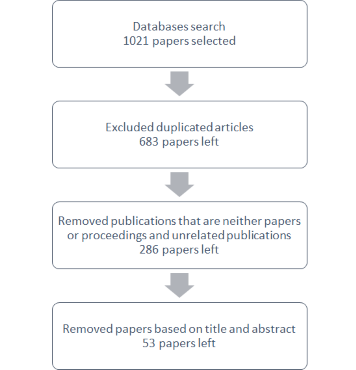
\includegraphics[]{imagens/paperScreening.png}
\end{figure}

The inclusion and exclusion criteria for those filters were defined as follows:

\noindent \textbf{Inclusion criteria:}
\begin{itemize}
    \item Articles describing the use of methods and that establish the relationship between machine learning and code smells.
    \item The studies publication type must be journals or conferences
\end{itemize}

\noindent \textbf{Exclusion criteria:}
\begin{itemize}
    \item Remove duplicates
    \item Remove studies where the code smells identification are done manually
    \item Remove non-empirical studies
\end{itemize}

\subsection{Quality assessment}

The main purpose of this study is to cover papers about the usage of Machine Learning Techniques for Code Smell identification. In order to try to avoid the non inclusion of relevant papers  precautions were taken. One of the cautions made was to include keywords, title, and abstract in the search, we also took the precaution of including synonyms and abbreviates.

Clear criteria for the exclusion and exclusion of the papers were also defined prior to the study. And each steps was registered so it could be evaluated by external parties. To assert the results of the study, peer reviews done by two graduated researchers were executed, compared and discussed in order to reach a consensus and avoid the perception of the researcher to influence the results. Criteria for classification was also selected from related works and explicit defined before the execution of the review.

The following questions were taken to improve the reliability of the work and avoid missing relevant papers:
\begin{itemize}
    \item \textbf{QA1}: Are the aims of the research defined explicitly?
    \item \textbf{QA2}: Is the context related to code smells?
    \item \textbf{QA3}: Are the used techniques exposed and related to Machine Learning?
    \item \textbf{QA4}: Is the experimental design appropriate and justifiable?
    \item \textbf{QA5}: Is the proposed estimation method comparable with other methods?
    \item \textbf{QA6}: Are the findings of study stated and supported by reporting results?
    \item \textbf{QA7}: Does the study add value to academia or industry community?
\end{itemize}